% LaTeX file for Chapter 03










\chapter{Results}

% 
% \section{Meta-analysis}
% The data at hand is composed of over 400,000 results with balanced sample size $n > 24$. The significance of the p-values of treatment effect estimates was calculated for all results in the dataset with acceptable sample size and outcome measures as odds ratios, peto odds ratios, risk ratios, risk differences and mean and standardized mean differences. 
% 
% %Significance over time? Chunck 1
% 
% The results that can be pooled are analysed by fixed-effects meta-analysis, random-effects meta-analysis and random-effects meta-analysis with Hartung-Knapp method.
% 
% \vspace{0mm}
% In the following, the results are combined with the results of their corresponding meta-analysis if possible (i.e. if studies were not unique in the dataset with respect to their experimental setup). The significance of the treatment effect (primary significance) in a single result is then compared to the significance of the pooled treatment effect (secondary significance). 
% In Figure \ref{primary.secondary.significance}, the overall fraction of studies with significant and non-significant meta-analysis results is shown. The meta-analysis method used to pool the treatment effect estimates and assessing significance is indicated on the right hand side of the Figure. The colors indicate the overall fraction of rejected or accepted null-hypotheses of no treatment effect.
% 
% \begin{figure}
% <<echo=FALSE, warning=FALSE>>=
% #plot(sig.meta.c)
% @
% \caption{Overall fraction of studies whose treatment effect estimate was significant when pooled by means of meta-analysis. The fractions have been calculated
% by fixed-effects, random-effects and Hartung and Knapp adjusted random-effects meta-analysis}
% \label{primary.secondary.significance}
% \end{figure}
% 
% What has been found is that even the meta-analysis that for all meta-analysis methods, the amount of secondary significance is higher than the amount of primary significance. Thus more primarily non-significant results can be attached to a secondarily significant result than vice-versa.
% 
% \vspace{0mm}
% To illustrate this, the fraction of studies with significant primary treatment effect and primary non-significant treatment effect can be plotted separately (Figure \ref{primary.secondary.significance.sep.sig}). 
% 
% \begin{figure}
% <<echo=FALSE, warning=FALSE>>=
% #grid.arrange(sig.meta.plot1, nonsig.meta.plot, ncol= 1)
% @
% \caption{Overall fraction of studies whose treatment effect estimate was significant when pooled by means of meta-analysis, separated by significance of study treatment effect estimate. The fractions have been calculated
% by fixed-effects, random-effects and Hartung and Knapp adjusted random-effects meta-analysis}
% \label{primary.secondary.significance}
% \end{figure}
% 
% It can be seen that the extent of overlap between primary and secondary significance varies between meta-analysis. A considerable amount of both primary significant and primary non-significant results are overruled by meta-analysis hypothesis tests. 
% 
% 
% The amount of significant heterogeneity in the results used by the meta-analyses is length(which(mly$sig.Q == 0)) and corresponds to (length(which(mly$sig.Q == 0))/ dim(mly)[1])*100\% of the total number of meta-analyses.
% 
% %Comparison of significance separated for significant Q? Chunck 2
% 
% %Proportion of significant pooled estimates based on proportion of single pooled estimates? Chunck 5


\section{Small study effects}



To provide an overview over the abundance of small study effects in the dataset, first it is shown how median absolute effect size decreases with increasing sample size of the results (Figure \ref{effect.samplesize}). 
%In some sense, this is the same idea as for a funnel plot, by depicting the size of effects relative to their variance. 

\vspace{0mm}
A clear trend of decrease of absolute effect size with increasing sample size (i.e. smaller variance) is visible. 
%It is particularly substantive from very small trials ($n$ = 10) to medium sample size ($n$ = 100) and afterwards it evens off. With increasing sample size, there are fewer results, therefore, the variation between medians increases. 
All effects are normalized by subtracting the mean effect size of the dataset and dividing through the standard deviation. Note that various types of outcome measures are included, such as mean difference and risk ratios, and are normalized with respect to all effects.

\begin{figure}
\begin{knitrout}
\definecolor{shadecolor}{rgb}{0.98, 0.98, 0.98}\color{fgcolor}

{\centering 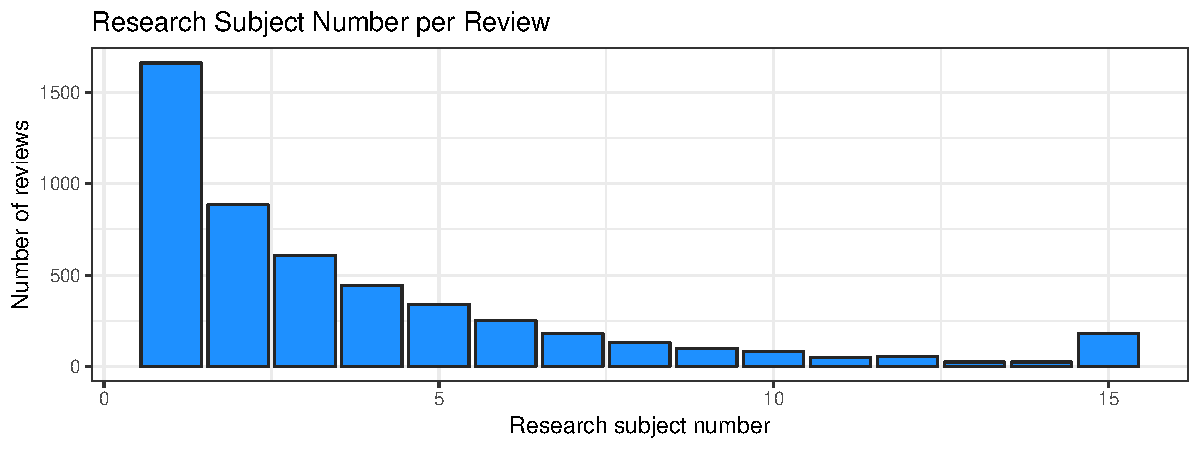
\includegraphics[width=\textwidth-3cm]{figure/ch02_figunnamed-chunk-5-1} 

}



\end{knitrout}
\caption{Median of the absolute value of the normalized effect size plotted against the total sample size.}
\label{effect.samplesize}
\end{figure}

The median absolute normalized effect size can be visualized for the different outcome measures separately (Figure \ref{effect.samplesize.separated}). The plot confirms the trend of median effect size decrease towards lower sample size (e.g. for Risk Ratios: decrease $> 0.1$ standard deviations from 10 to 50 study participants). Instead of normalizing the effects 
%(i.e. subtracting mean and dividing through the standard deviation) 
for all effect sizes, the effects are normalized with respect to the effects of the same outcome measures. 

\begin{figure}
\begin{knitrout}
\definecolor{shadecolor}{rgb}{0.98, 0.98, 0.98}\color{fgcolor}

{\centering 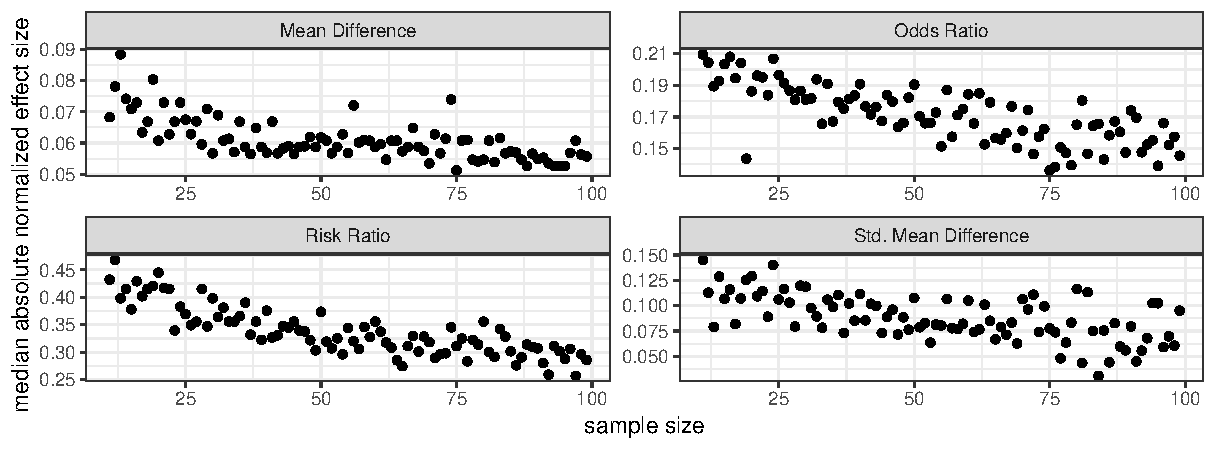
\includegraphics[width=\textwidth-3cm]{figure/ch02_figunnamed-chunk-6-1} 

}



\end{knitrout}
\caption{Median of the absolute value of the normalized effect size plotted against the total sample size, separated for outcome measures.}
\label{effect.samplesize.separated}
\end{figure}

%Show absolute effect size depending on scaled time? Chunck 3




\subsection{Small Study Effect Tests}



There are tests that can be applied to find out if small study effects are present in the meta analysis. For the precise description, see the methods section. Application of the tests is only recommended if there are ten or more studies \citep{cochrane.handbook} that can be used, so all meta-analyses with less than ten studies have been excluded.

\vspace{0mm}
There are modifications to make tests more appropriate in case of binary outcomes, therefore the results have been separated in continuous and dichotomous outcome test results. In Figure \ref{bias.results.cont} the proportion of test results that led to rejection of the null hypothesis of no small study effect based on the 5 \% level are shown for continuous outcomes ($n$ = 1383)
The same is shown in Figure \ref{bias.results.bin} for dichotomous outcome measures ($n$ = 3955). The amount of studies varies from 5\% (Schwarzer's Test) to 13 \% (Egger's Test) for binary outcomes and 9\% (Begg and Mazumdar's Test) to 25 \% (Egger's Test) for continuous outcomes. 


\begin{figure}
\begin{knitrout}
\definecolor{shadecolor}{rgb}{0.98, 0.98, 0.98}\color{fgcolor}

{\centering 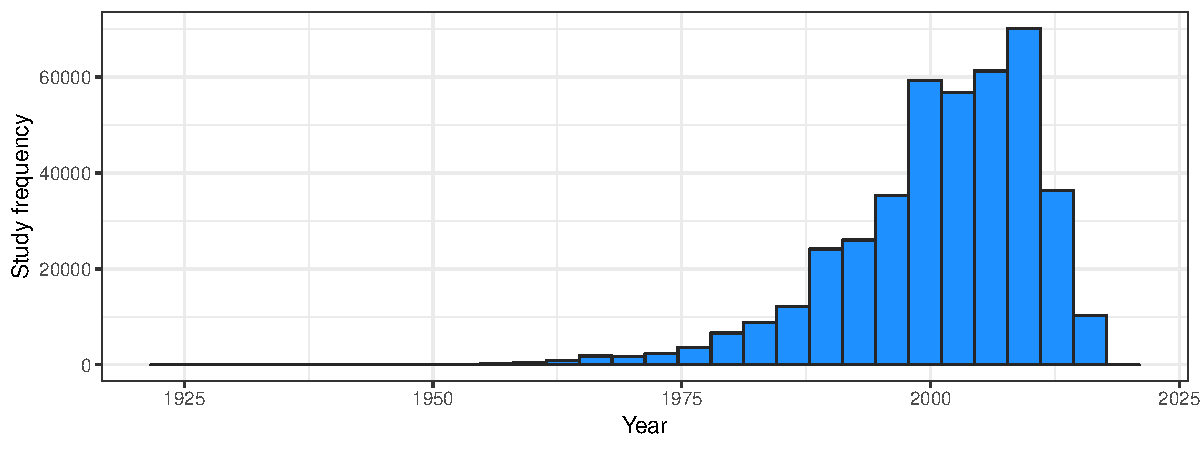
\includegraphics[width=\textwidth-3cm]{figure/ch02_figunnamed-chunk-8-1} 

}



\end{knitrout}
\caption{Proportion where the null hypothesis of no small study effect is rejected based on the 5\% significance level for different tests (continuous outcomes).}
\label{bias.results.cont}
\end{figure}

\begin{figure}
\begin{knitrout}
\definecolor{shadecolor}{rgb}{0.98, 0.98, 0.98}\color{fgcolor}

{\centering 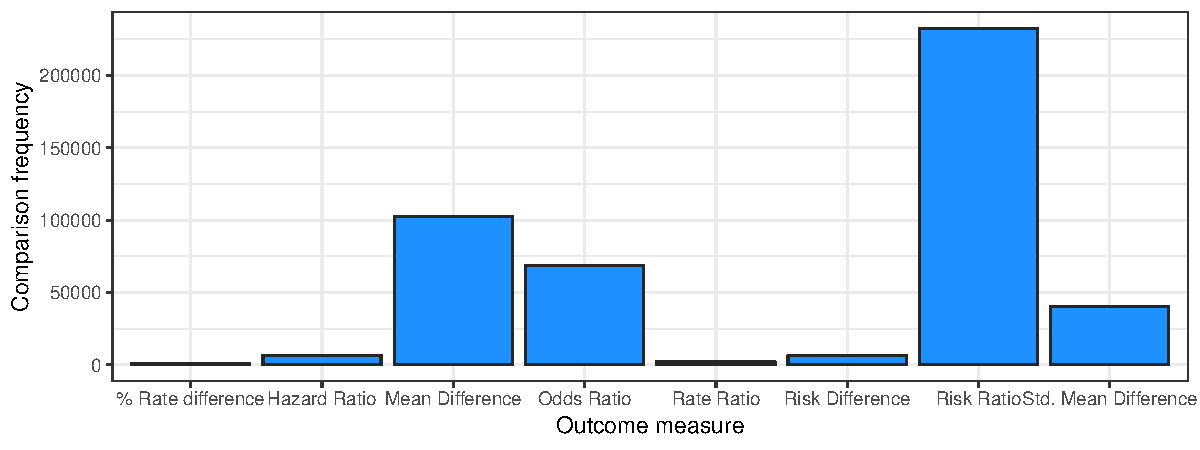
\includegraphics[width=\textwidth-3cm]{figure/ch02_figunnamed-chunk-9-1} 

}



\end{knitrout}
\caption{Proportion where the null hypothesis of no small study effect is rejected based on the 5\% significance level for different tests (dichotomous outcomes).}
\label{bias.results.bin}
\end{figure}

There is no substantive change in the fraction of positive test results, depending on if the pooled treatment effect size estimate is significant or not. Most substantively, the fraction of positive Egger Test results increases for significant pooled treatment effects by 0.1825716 (the minimal increase is -0.0032246 for Schwarzer's Test).

%Show plots of significant meta-analyses separated? Chunck 4

Furthermore one can look if the frequencies of tests that reject the null hypotheses change over time (mean publication year of the studies included in the meta analyses). The proportion of the test results are shown in Figure \ref{pub.bias.time.overtime}. The Figure suggests that the frequency of publication bias remains constant over time. The mean publication years have been restricted such that at least 180 meta-analyses are available per year, such that random fluctuation is restricted to some extent. The significance threshold for the $p$-values used is 0.05, and the small study effect test used is Thomson's test (with the arcsine variance stabilizing transformation function used in the case of binary outcomes).

\begin{figure}
\begin{knitrout}
\definecolor{shadecolor}{rgb}{0.98, 0.98, 0.98}\color{fgcolor}

{\centering 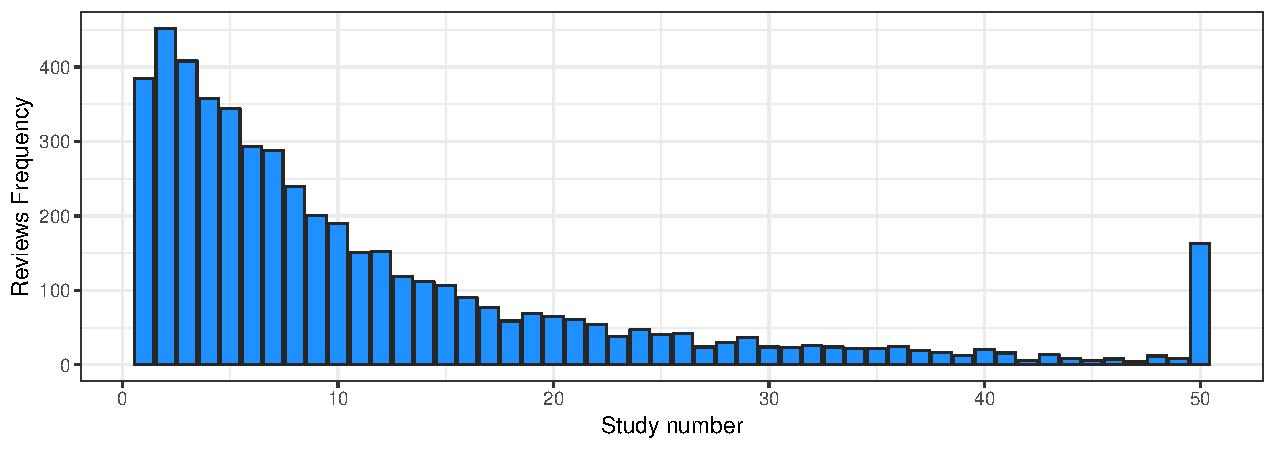
\includegraphics[width=\textwidth-3cm]{figure/ch02_figunnamed-chunk-10-1} 

}



\end{knitrout}
\caption{Proportion of test results where the null hypothesis of no small study effect is rejected over time (mean publication.year).}
\label{pub.bias.overtime}
\end{figure}


The agreement of the tests, i.e. the proportion of meta-analyses where the rest results are equal between tests, is shown in Table \ref{agreement.bin} and Table \ref{agreement.cont}, again separated for outcome types. Agreement in tests for binary outcomes is better than continuous outcomes, with some variation between tests (binary outcomes: 83 to 91\%). Correlation varies more between tests, both for continuous and binary outcome tests.

% latex table generated in R 3.5.1 by xtable 1.8-3 package
% Tue May 21 16:11:40 2019
\begin{table}[ht]
\centering
\begingroup\footnotesize
\begin{tabular}{lll}
  \hline
 & Test Agreement & P-value Correlation \\ 
  \hline
egger.schwarzer & 0.73 & 0.23 \\ 
  egger.peter & 0.75 & 0.37 \\ 
  egger.rucker & 0.75 & 0.34 \\ 
  egger.harbord & 0.79 & 0.51 \\ 
  schwarzer.peter & 0.81 & 0.26 \\ 
  schwarzer.rucker & 0.81 & 0.25 \\ 
  schwarzer.harbord & 0.86 & 0.47 \\ 
  rucker.peter & 0.87 & 0.64 \\ 
  harbord.peter & 0.84 & 0.50 \\ 
   \hline
\end{tabular}
\endgroup
\caption{Proportion of tests that agree in rejection ar acceptance of the null hypothesis that there is no small study effect (dichotomous outcomes)} 
\label{agreement.bin}
\end{table}



% latex table generated in R 3.5.1 by xtable 1.8-3 package
% Tue May 21 16:11:40 2019
\begin{table}[ht]
\centering
\begingroup\footnotesize
\begin{tabular}{lll}
  \hline
 & Test Agreement & P-value Correlation \\ 
  \hline
thomson.egger & 0.85 & 0.69 \\ 
  thomson.begg & 0.77 & 0.47 \\ 
  egger.begg & 0.73 & 0.36 \\ 
   \hline
\end{tabular}
\endgroup
\caption{Proportion of tests that agree in rejection ar acceptance of the null hypothesis that there is no small study effect (continuous outcomes)} 
\label{agreement.cont}
\end{table}


\vspace{0mm}
Test performance depends on the sample size, despite having restricted sample size to a minimum of 10 studies. The p-values of the Thompson and Sharp tests are shown with respect to the sample size of the meta-analysis in Figure \ref{pvalues.samplesize}. %(Suggests that 10 is likely too small)
In the case of binary outcomes, the arcsine variance stabilizing function has been applied prior to use of Thompson and Sharp's test. A trend towards more rejections for larger sample sizes can be seen.

\begin{figure}
\begin{knitrout}
\definecolor{shadecolor}{rgb}{0.98, 0.98, 0.98}\color{fgcolor}

{\centering 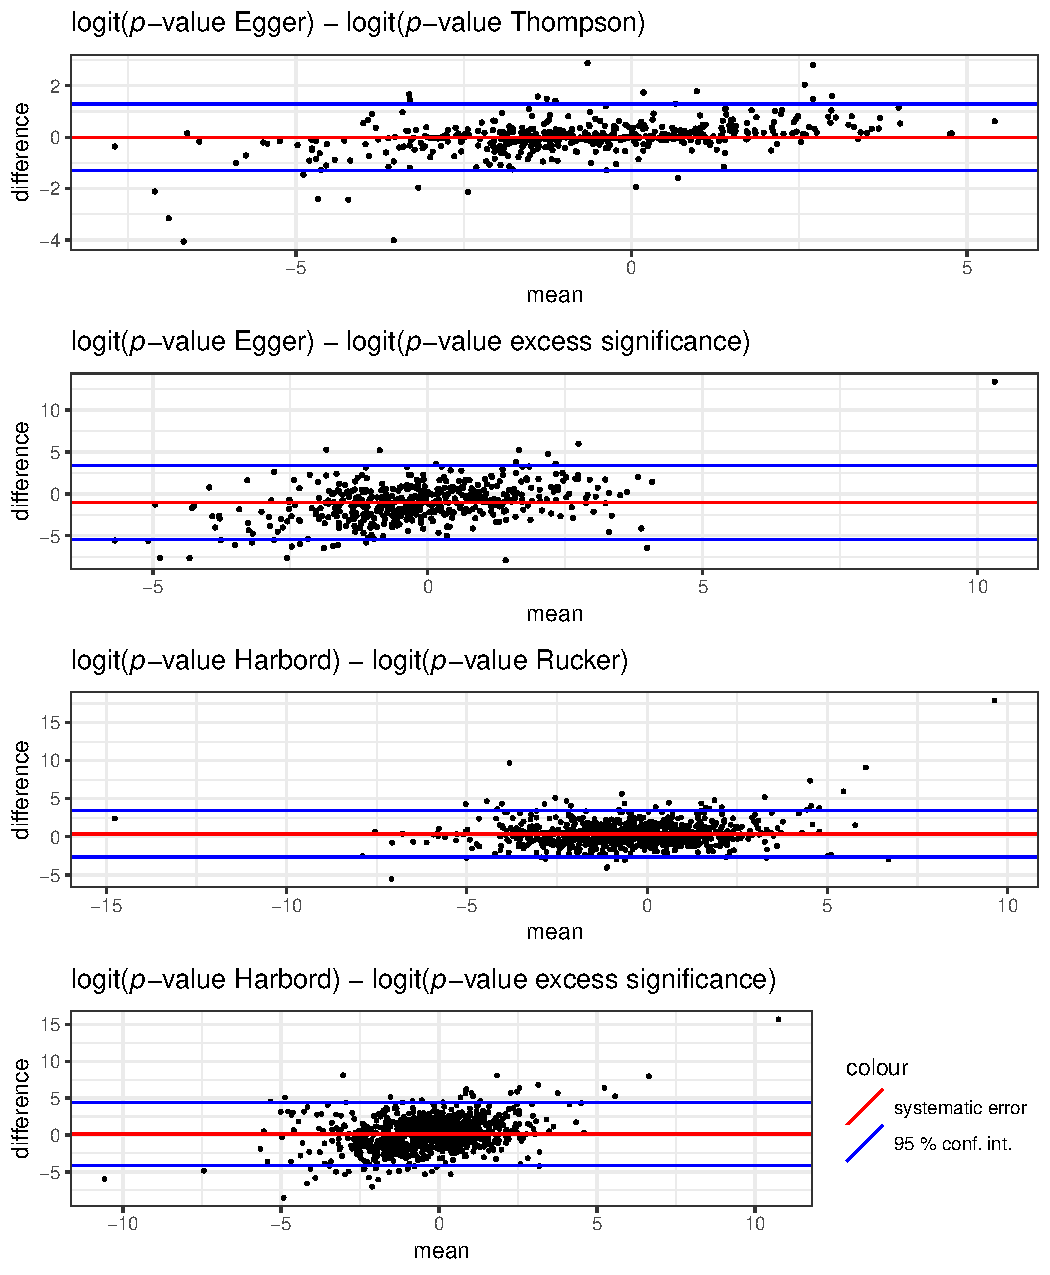
\includegraphics[width=\textwidth-3cm]{figure/ch02_figunnamed-chunk-13-1} 

}



\end{knitrout}
\caption{P-values of Thomson and Sharp's test for small study effects and their corresponding sample size.}
\label{pvalues.samplesize}
\end{figure}



\vspace{0mm}
One can use the proportion of added studies by the trim-and-fill method from the overall number of studies to further investigate the extent of small study effects. The mean fraction of trimmed comparisons for binary outcomes is 0.19 and the median 0.18. 
% A histogram with those fractions is shown in Figure \ref{trimfill.cont} for continuous outcomes and \ref{trimfill.bin} for dichotomous outcomes. In both cases, the method very commonly adds supposedly unpublished studies to the meta-analyses. 
In Figure \ref{trimfill.pvalues.bin} and Figure \ref{trimfill.pvalues.cont}, the relationship between fraction of added studies by trim-and-fill and the hypothesis test decisions of the small study effects tests is shown for continuous and dichotomous outcomes. In the case of Peters test dor dichotomous outcomes, there is less agreement with the trim-and fill method than in the case of Thomson and Sharp's test for continuos outcomes in the sense that the fraction of meta-analyses with rejected null hypothesises increases more clearly when there are more studies added by trim-and-fill. 

\begin{figure}
\begin{knitrout}
\definecolor{shadecolor}{rgb}{0.98, 0.98, 0.98}\color{fgcolor}

{\centering 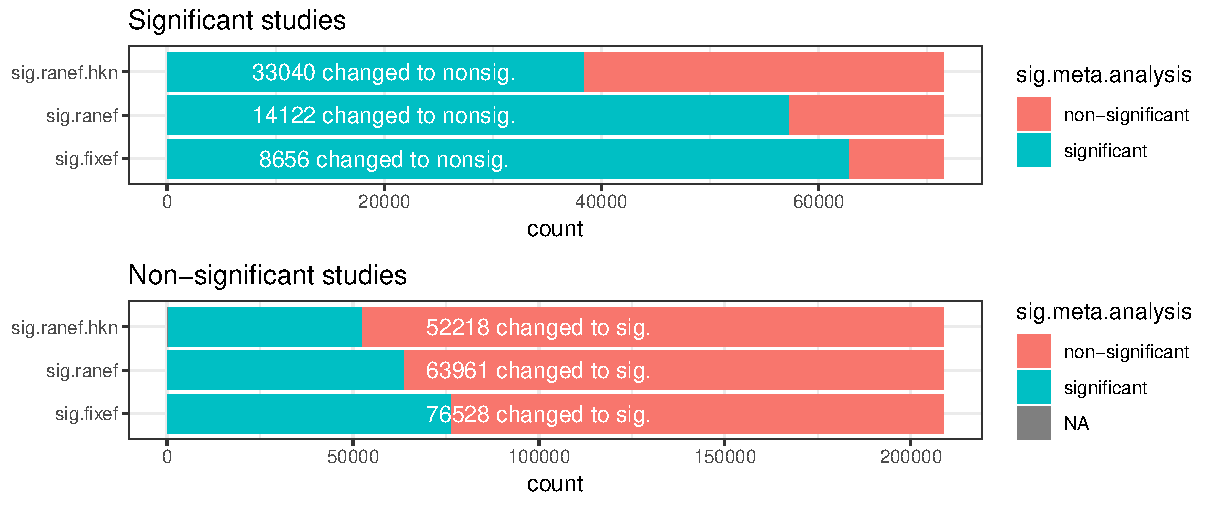
\includegraphics[width=\textwidth-3cm]{figure/ch02_figunnamed-chunk-14-1} 

}



\end{knitrout}
\caption{Fraction of added studies for small study effect correction by trim and fill and the corresponding small study effect test decision (based on 5\% significance level) of Peters test and dichotomous outcomes}
\label{trimfill.pvalues.bin}
\end{figure}

\begin{figure}
\begin{knitrout}
\definecolor{shadecolor}{rgb}{0.98, 0.98, 0.98}\color{fgcolor}

{\centering 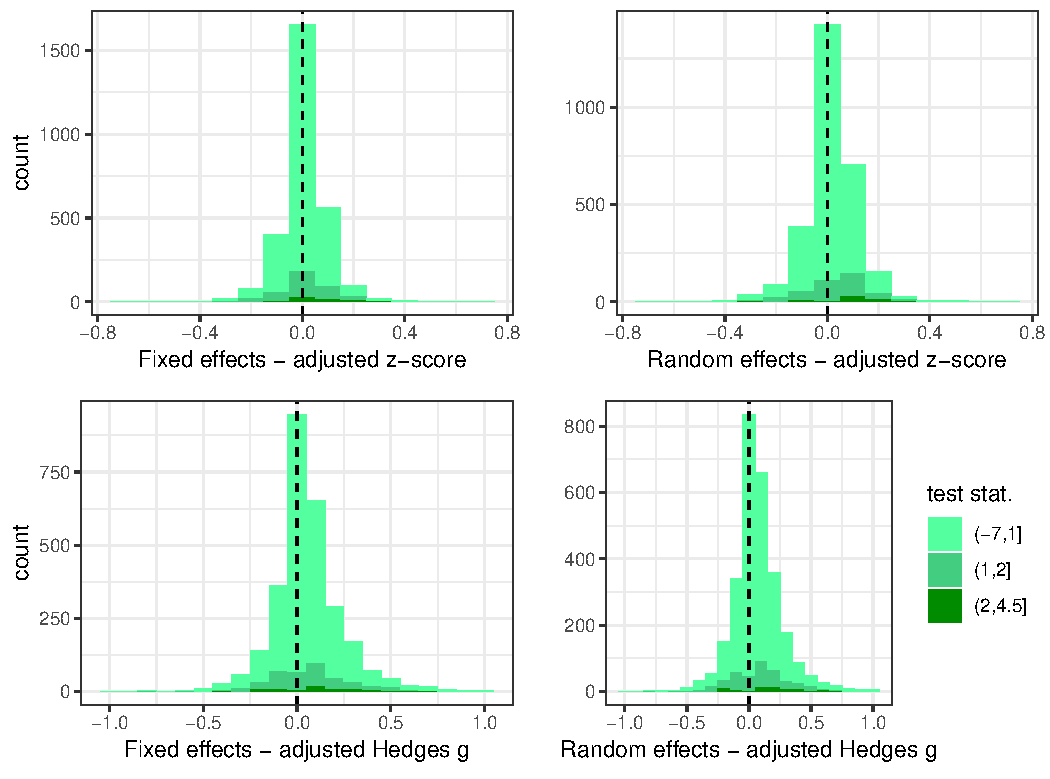
\includegraphics[width=\textwidth-3cm]{figure/ch02_figunnamed-chunk-15-1} 

}



\end{knitrout}
\caption{Fraction of added studies for small study effect correction by trim and fill and the corresponding small study effect test decision (based on 5\% significance level) of Thomson and Sharp's test and continuous outcomes}
\label{trimfill.pvalues.cont}
\end{figure}


\subsection{Small Study Effect Correction}
Multiple methods are available to correct for the effects of small study effects in order to get an unbiased estimate. Three of them will be applied to the meta-analyses shown previously that have ten or more study results and are therefore eligible for testing for publication bias. 

\vspace{0mm}
The extent to what the results of the meta-analysis results are changed can be investigated. Because statistical significance is often used to decide if there is a treatment effect, a non-significant corrected effect size estimate can indicate that an observed treatment effect has been accepted because of small study effects. Therefore, the cases have been counted in which 
\begin{enumerate}
\item Significance or non-significance of pooled estimate of meta-analysis did not change after correction for small study effects.
\item Significance of pooled estimate of meta-analysis did change to non-significance after correction for small study effects.
\item Non-significance of pooled estimate of meta-analysis did change to significance after correction for small study effects.
\end{enumerate}

The results of this can be seen in Figure \ref{significance.change.fixed} for all three methods, comparing the significance of the corrected pooled effect size estimate with the significance of the pooled effect size estimate of the fixed effects meta-analysis. The same for significance of random effects meta-analysis is shown in Figure \ref{significance.change.random}. The significance threshold was chosen such that the $p$-value had to be < 0.05 for rejection of the null hypothesis of no treatment effect. The correction methods were trim-and-fill, copas selection model and regression with random effects and shrinkage of within-study-variance methods. More details to the applied correction methods and their application are in the methods section \ref{methods}. Notably, the correction methods has been applied to all meta-analyses, thus also for such that had no significant small study effect test result. 


\begin{figure}
\begin{knitrout}
\definecolor{shadecolor}{rgb}{0.98, 0.98, 0.98}\color{fgcolor}

{\centering 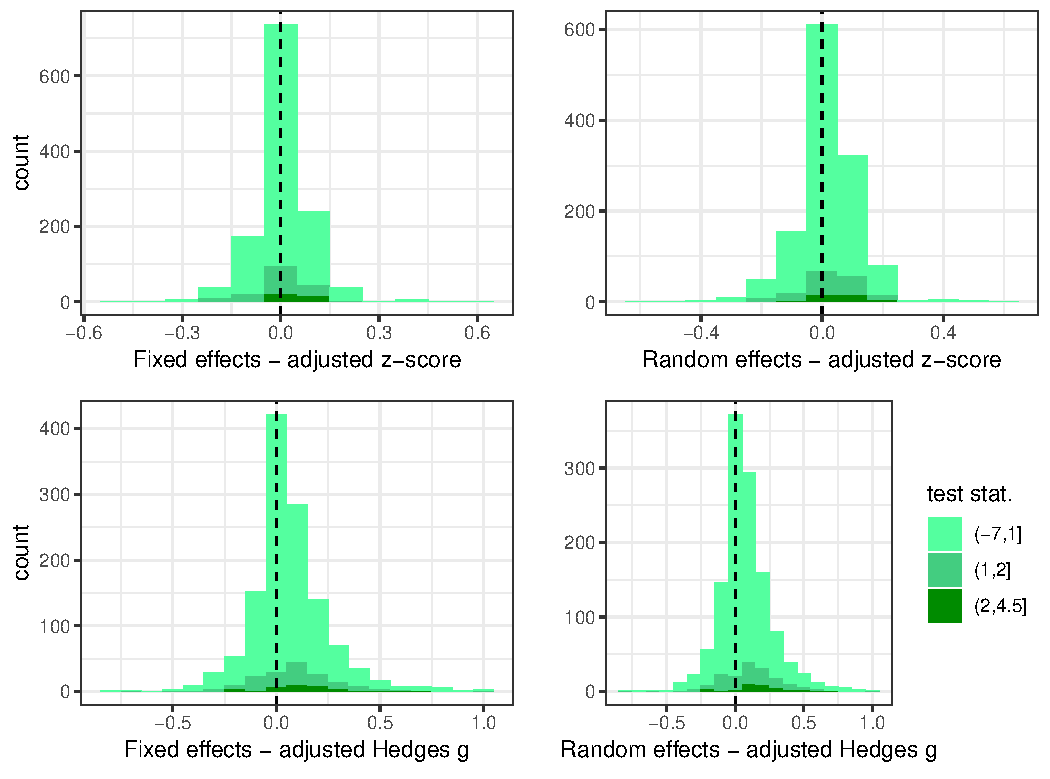
\includegraphics[width=\textwidth-3cm]{figure/ch02_figunnamed-chunk-16-1} 

}



\end{knitrout}
\caption{Change in signficance of fixed effects meta-analysis pooled estimate after correction.}
\label{significance.change.fixed}
\end{figure}

\begin{figure}
\begin{knitrout}
\definecolor{shadecolor}{rgb}{0.98, 0.98, 0.98}\color{fgcolor}

{\centering 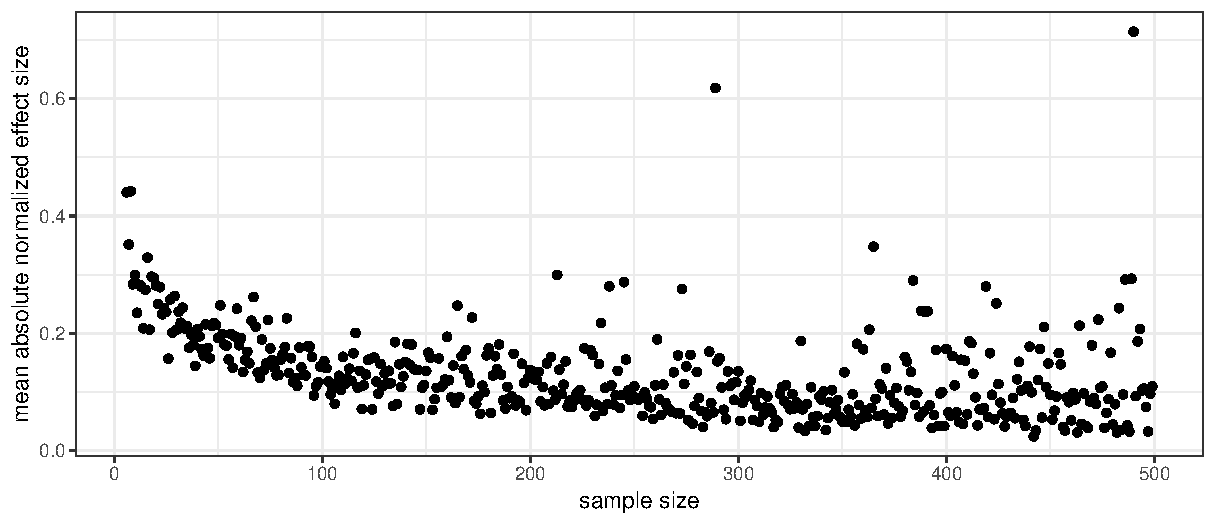
\includegraphics[width=\textwidth-3cm]{figure/ch02_figunnamed-chunk-17-1} 

}



\end{knitrout}
\caption{Change in signficance of random effects meta-analysis pooled estimate after correction.}
\label{significance.change.random}
\end{figure}

Since it has been previously seen in Figure \ref{test.results} that the results of small study effects vary considerably between continuous outcomes, the results in significance change from fixed effects meta-analysis can be seen separately in Figure \ref{significance.change.fixed.sep} for continuous and binary outcomes. The change in significance from random effects meta-analysis to significance of corrected estimate can be seen in Figure \ref{significance.change.fixed.sep}

\begin{figure}
\begin{knitrout}
\definecolor{shadecolor}{rgb}{0.98, 0.98, 0.98}\color{fgcolor}

{\centering 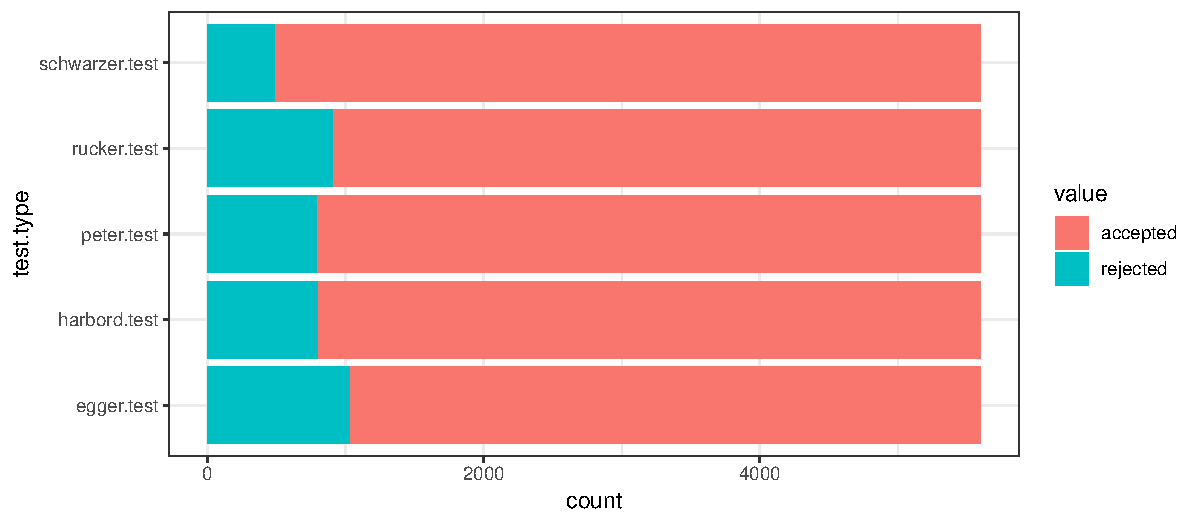
\includegraphics[width=\textwidth-3cm]{figure/ch02_figunnamed-chunk-18-1} 

}



\end{knitrout}
\caption{Change in signficance of fixed effects meta-analysis pooled estimate after correction, separated for continuous and binary outcomes.}
\label{significance.change.fixed.sep}
\end{figure}

\begin{figure}
\begin{knitrout}
\definecolor{shadecolor}{rgb}{0.98, 0.98, 0.98}\color{fgcolor}

{\centering 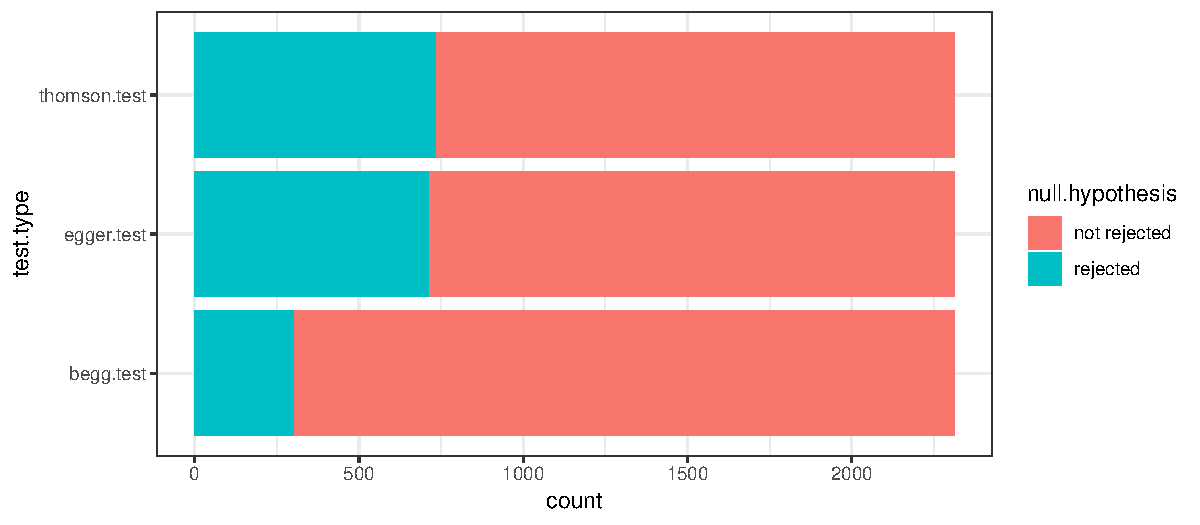
\includegraphics[width=\textwidth-3cm]{figure/ch02_figunnamed-chunk-19-1} 

}



\end{knitrout}
\caption{Change in signficance of random effects meta-analysis pooled estimate after correction, separated for continuous and binary outcomes.}
\label{significance.change.random}
\end{figure}

Because the real amount of publication bias in the dataset is not known, the correction method can also be applied only to meta-analyses that have publication bias according to the small study effect tests in the previous section. Because the test developed by \citet{thomson.sharp} has been applied to both binary and continuous outcome meta-analyses (in the case of binary outcomes to arcsine variance stabilized proportions), it is used as a criterium to distinguish biased from unbiased meta-analyses. The proportions of significance tests of pooled treatment effects that turned from significant to non-significant, non-significant to significant etc. are shown in Figure \ref{significance.change.fixed.sep}. Fixed effects meta-analysis has been used to determine signficance of the uncorrected estimate.


\begin{figure}
\begin{knitrout}
\definecolor{shadecolor}{rgb}{0.98, 0.98, 0.98}\color{fgcolor}

{\centering 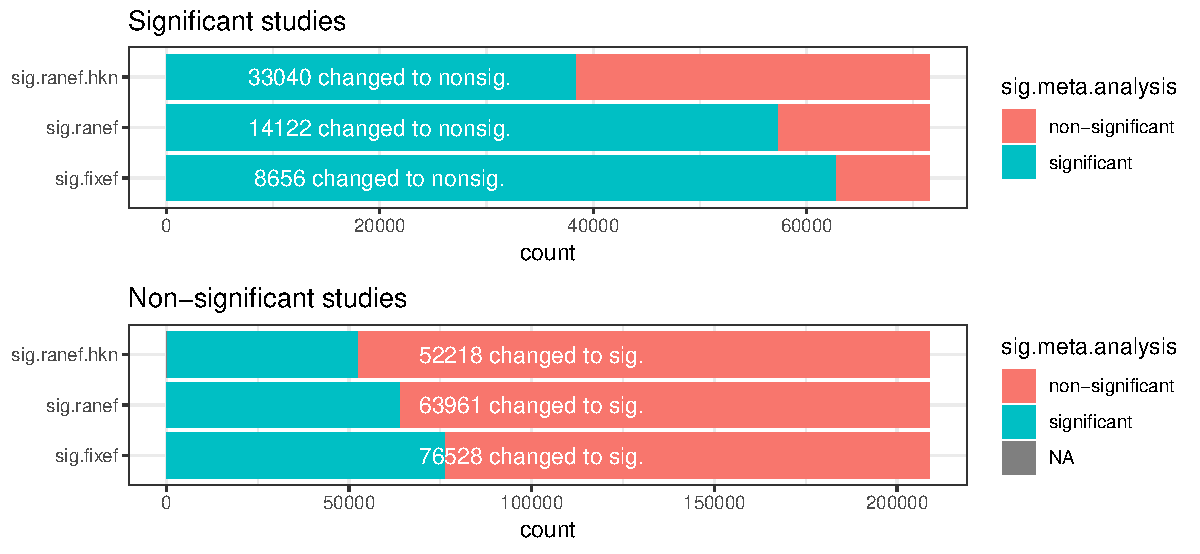
\includegraphics[width=\textwidth-3cm]{figure/ch02_figunnamed-chunk-20-1} 

}



\end{knitrout}
\caption{Change in signficance of random effects meta-analysis pooled estimate after correction, separated for continuous and binary outcomes.}
\label{significance.change.random}
\end{figure}

Similarly, the number of missing studies per meta-analysis, i.e. those which have not been included because of small study effects, are estimated by the copas and trim-and-fill method and their empirical distribution is shown in histograms in Figure \ref{missing.studies.distribution}. For visualisation, the fraction of unpublished studies from the total fraction of available studies is shown.

\begin{figure}
\begin{knitrout}
\definecolor{shadecolor}{rgb}{0.98, 0.98, 0.98}\color{fgcolor}

{\centering 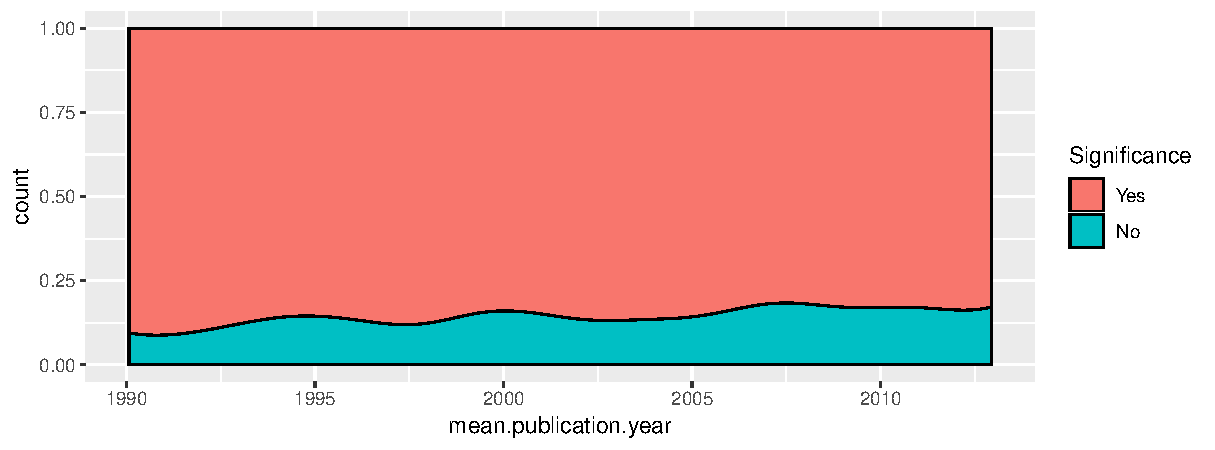
\includegraphics[width=\textwidth-3cm]{figure/ch02_figunnamed-chunk-21-1} 

}



\end{knitrout}
\caption{Fraction of missing studies estimated of the number of total studies included in the meta-analysis for copas selection and trim-and-fill method.}
\label{missing.studies.distribution}
\end{figure}




% # <<results = 'asis', Echo = FALSE>>=
% # rejection.bin <- meta.bin %>% summarize(egger.rejection = mean(egger.test),
% #                                             schwarzer.rejection = mean(schwarzer.test),
% #                                             rucker.rejection = mean(rucker.test),
% #                                             harbord.rejection = mean(harbord.test),
% #                                             peter.rejection = mean(peter.test))
% # print(xtable(rejection.bin), label = "bias.results", caption = "Cumulative number of groups with number of reproduction trials >= n", align = "llll", digits = 0), include.rownames = F, size = "footnotesize")
% # @






% 
% For continuous outcomes, three tests are available: Eggers (based on linear regression), Thompson and Sharp (weighted linear regression) and Begg and Mazumdar (rank based) test. The following three figures show the distribution of p-values of the corresponding tests. Note that only meta analyses with more than 10 comparisons have been included. 
% 
% \vspace{0mm}
% Since each histogram of p-values has 20 bins, the content of the bin with the smallest p-values is equal to the number of meta-analyses whose reporting bias test reports a p-value < 0.05. The fraction of those analyses in which we would reject the null-hypothesis based on the 5 \% threshold can therefore be assessed by eye, and would be for example for Eggers test somewhat less than one third of all analyses. 
% 
% \begin{figure}
% <<echo=FALSE>>=
% data %>% filter(outcome.measure == "Mean Difference" | outcome.measure == "Std. Mean Difference") %>% #filter(file.nr < 503) %>% 
%   filter(sd1 > 0 & sd2 > 0 ) %>% filter(!is.na(sd1) & !is.na(sd2)) %>% 
%   filter(mean1 != 0 | mean2 != 0 ) %>% filter(!is.na(mean1) & !is.na(mean2)) %>% 
%   group_by(file.nr, outcome.nr, subgroup.nr) %>% 
%   mutate(n = n()) %>% filter(n > 9) %>% 
%   summarize(pval = metabias(metacont(n.e = total1, mean.e = mean1, sd.e = sd1, n.c = total2, mean.c = mean2, sd.c = sd2), 
%                             method = "linreg")$p.val) %>% 
%   ggplot(aes(x = pval)) + geom_histogram(col = "gray15", fill = "dodgerblue", bins = 20) +
%   theme_bw() + labs(title = "Eggers Reporting Bias Test P-values for Continuous Outcome Meta-Analyses") + xlab("P-value") + ylab("Frequency")
% @
% \caption{Histogram of p-values for Eggers reporting bias test (linear regression based) for continuous outcome meta analysis.}
% \label{egger.cont}
% \end{figure}
% 
% 
% \begin{figure}
% <<echo=FALSE>>=
% data %>% filter(outcome.measure == "Mean Difference" | outcome.measure == "Std. Mean Difference") %>% #filter(file.nr < 503) %>% 
%   filter(sd1 > 0 & sd2 > 0 ) %>% filter(!is.na(sd1) & !is.na(sd2)) %>% 
%   filter(mean1 != 0 | mean2 != 0 ) %>% filter(!is.na(mean1) & !is.na(mean2)) %>% 
%   group_by(file.nr, outcome.nr, subgroup.nr) %>% 
%   mutate(n = n()) %>% filter(n > 9) %>% 
%   summarize(pval = metabias(metacont(n.e = total1, mean.e = mean1, sd.e = sd1, n.c = total2, mean.c = mean2, sd.c = sd2), 
%                             method = "mm")$p.val) %>% 
%   ggplot(aes(x = pval)) + geom_histogram(col = "gray15", fill = "dodgerblue", bins = 20) +
%   theme_bw() + labs(title = "Thomson Sharp Reporting Bias Test P-values for Continuous Outcome Meta-Analyses") + xlab("P-value") + ylab("Frequency")
% @
% \caption{Histogram of p-values for Thompsom and Sharp reporting bias test (weighted linear regression based) for continuous outcome meta analysis.}
% \label{thomson.cont}
% \end{figure}
% 
% \begin{figure}
% <<echo=FALSE>>=
% data %>% filter(outcome.measure == "Mean Difference" | outcome.measure == "Std. Mean Difference") %>% #filter(file.nr < 503) %>% 
%   filter(sd1 > 0 & sd2 > 0 ) %>% filter(!is.na(sd1) & !is.na(sd2)) %>% 
%   filter(mean1 != 0 | mean2 != 0 ) %>% filter(!is.na(mean1) & !is.na(mean2)) %>% 
%   group_by(file.nr, outcome.nr, subgroup.nr) %>% 
%   mutate(n = n()) %>% filter(n > 9) %>% 
%   summarize(pval = metabias(metacont(n.e = total1, mean.e = mean1, sd.e = sd1, n.c = total2, mean.c = mean2, sd.c = sd2), 
%                             method = "rank")$p.val) %>% 
%   ggplot(aes(x = pval)) + geom_histogram(col = "gray15", fill = "dodgerblue", bins = 20) +
%   theme_bw() + labs(title = "Begg and Mazumdar Reporting Bias Test P-values for Continuous Outcome Meta-Analyses") + xlab("P-value") + ylab("Frequency")
% @
% \caption{Histogram of p-values for Begg and Mazumdar reporting bias test (rank based) for continuous outcome meta analysis.}
% \label{begg.cont}
% \end{figure}
% 
% 
% For binary outcomes, Peters and Harbords reporting bias test have been chosen. Also here, only meta-analyses with more than 10 comparisons are included.
% 
% \begin{figure}
% <<echo=FALSE>>=
% data %>% filter(outcome.measure == "Risk Ratio" | outcome.measure == "Odds Ratio") %>% filter(file.nr != 3014) %>% 
%   filter(events1 > 0 | events2 > 0) %>% 
%   filter(total1 - events1 > 0 | total2 - events2 > 0) %>%
%   group_by(file.nr, outcome.nr, subgroup.nr) %>% 
%   mutate(n = n()) %>% filter(n > 9) %>% 
%   summarize(pval = metabias(metabin(event.e = events1, n.e = total1, event.c = events2, n.c = total2, sm = "OR"), method = "peters")$p.val) %>% 
%   ggplot(aes(x = pval)) + geom_histogram(col = "gray15", fill = "dodgerblue", bins = 20) +
%   theme_bw() + labs(title = "Peters Reporting Bias Test P-values for Binary Outcome Meta-Analyses") + xlab("P-value") + ylab("Frequency")
% @
% \caption{Histogram of p-values for Peters reporting bias test (rank based) for continuous outcome meta analysis.}
% \label{peters.bin}
% \end{figure}
% 
% 
% \begin{figure}
% <<echo=FALSE>>=
% data %>% filter(outcome.measure == "Risk Ratio" | outcome.measure == "Odds Ratio") %>% filter(file.nr != 3014) %>% 
%   filter(events1 > 0 | events2 > 0) %>% 
%   filter(total1 - events1 > 0 | total2 - events2 > 0) %>%
%   group_by(file.nr, outcome.nr, subgroup.nr) %>% 
%   mutate(n = n()) %>% filter(n > 9) %>% 
%   summarize(pval = metabias(metabin(event.e = events1, n.e = total1, event.c = events2, n.c = total2, sm = "OR"), method = "score")$p.val) %>% 
%   ggplot(aes(x = pval)) + geom_histogram(col = "gray15", fill = "dodgerblue", bins = 20) +
%   theme_bw() + labs(title = "Harbord Reporting Bias Test P-values for Binary Outcome Meta-Analyses") + xlab("P-value") + ylab("Frequency")
% @
% \caption{Histogram of p-values for Harbord reporting bias test (rank based) for continuous outcome meta analysis.}
% \label{harbord.bin}
% \end{figure}


%%%%%%%%%%%%%%%%%%%%%%%%%%%%%%%%%%%%%%%%%%%%%%%%%%%%%%%%%%%%%%%%%%%%%%%%%%%%%%%%%%%%%%%%%%%%%%%%%%%%%%%%%%%%%%%%%%%%%%%%
%Chunck 1
%%%%%%%%%%%%%%%%%%%%%%%%%%%%%%%%%%%%%%%%%%%%%%%%%%%%%%%%%%%%%%%%%%%%%%%%%%%%%%%%%%%%%%%%%%%%%%%%%%%%%%%%%%%%%%%%%%%%%%%%
%%%%%%%%%%%%%%%%%%%%%%%%%%%%%%%%%%%%%%%%%%%%%%%%%%%%%%%%%%%%%%%%%%%%%%%%%%%%%%%%%%%%%%%%%%%%%%%%%%%%%%%%%%%%%%%%%%%%%%%%

% Since most of the times the study publication year is available for a given result, the fraction of significant treatment effects found is shown over time in Figure \ref{study.significance.overtime}. The $p$-value was chosen to be 0.05  only times where a reasonbly large number of effect estimates is available is shown in order to reduce random fluctuation ($n$ > 800). 
% 
% \begin{figure}
% <<echo=FALSE, warning=FALSE>>=
% data.ext %>% filter(!is.na(sig.type)) %>%  ggplot(aes(x = study.year, fill = factor(sig.type), stat(count))) + geom_density(na.rm = T, position = "fill") + 
%   labs(fill = "Significance") + scale_fill_discrete(labels= c("Yes", "No"))+ scale_x_continuous(limits = c(1970, 2017))
% @
% \caption{Mean of the absolute value of the normalized effect size plotted against the total sample size.}
% \label{study.significance.overtime}
% \end{figure}

%%%%%%%%%%%%%%%%%%%%%%%%%%%%%%%%%%%%%%%%%%%%%%%%%%%%%%%%%%%%%%%%%%%%%%%%%%%%%%%%%%%%%%%%%%%%%%%%%%%%%%%%%%%%%%%%%%%%%%%%
%Chunck 2
%%%%%%%%%%%%%%%%%%%%%%%%%%%%%%%%%%%%%%%%%%%%%%%%%%%%%%%%%%%%%%%%%%%%%%%%%%%%%%%%%%%%%%%%%%%%%%%%%%%%%%%%%%%%%%%%%%%%%%%%
%%%%%%%%%%%%%%%%%%%%%%%%%%%%%%%%%%%%%%%%%%%%%%%%%%%%%%%%%%%%%%%%%%%%%%%%%%%%%%%%%%%%%%%%%%%%%%%%%%%%%%%%%%%%%%%%%%%%%%%%

% The separation of studies can also be made based on the significance of heterogeneity between them when pooling them by means of a meta-analysis. Significant heterogeneity between studies corresponds to a rejection of the null-hypothesis that all the study treatment effect estimates share the same underlying distribution. The test used to assess heterogeneity was based on the between-study heterogeneity estimate $Q$ estimated as \citet{tau.estimator} suggested. This is shown in Figure \ref{primary.secondary.significance.sep.sig}.
% 
% \begin{figure}
% <<echo=FALSE, warning=FALSE>>=
% grid.arrange(sig.meta.Q1, nonsig.meta.Q, ncol= 1)
% @
% \caption{Overall fraction of studies whose treatment effect estimate was significant when pooled by means of meta-analysis, separated by significance of study treatment effect estimate. The fractions have been calculated
% by fixed-effects, random-effects and Hartung and Knapp adjusted random-effects meta-analysis}
% \label{primary.secondary.significance.sep.sig}
% \end{figure}

%%%%%%%%%%%%%%%%%%%%%%%%%%%%%%%%%%%%%%%%%%%%%%%%%%%%%%%%%%%%%%%%%%%%%%%%%%%%%%%%%%%%%%%%%%%%%%%%%%%%%%%%%%%%%%%%%%%%%%%%
%Chunck 3
%%%%%%%%%%%%%%%%%%%%%%%%%%%%%%%%%%%%%%%%%%%%%%%%%%%%%%%%%%%%%%%%%%%%%%%%%%%%%%%%%%%%%%%%%%%%%%%%%%%%%%%%%%%%%%%%%%%%%%%%
%%%%%%%%%%%%%%%%%%%%%%%%%%%%%%%%%%%%%%%%%%%%%%%%%%%%%%%%%%%%%%%%%%%%%%%%%%%%%%%%%%%%%%%%%%%%%%%%%%%%%%%%%%%%%%%%%%%%%%%%

% A second way to analyse meta-analyses is a cumulative meta-analysis that should reveal shifts in treatment effect sizes over time. This can again be done for the entire dataset, i.e. for all effect estimates and their ordering in time. It is important to scale the effect estimates here with respect to the estimates of the replication studies that are about the same subject, have the same outcome measure, etc. Also, only effect estimates that can be compared to other estimates before are included, i.e. only study results with one or more replica are included. Time needs to be scaled and normalized in order to compare multiple time-trends in effect size to each other and gain insights in the overall trend. This is done in Figure \ref{effects.overtime.separated}, separared for odds rati, risk ratio, and mean and standardized difference outcome measures. In order to reduce the spread over time of effect sizes, only studies between 1970 and 2019 were included, as well as studies with a minimal group size of 12 participants (each group).
% 
% \begin{figure}
% <<echo=FALSE>>=
% data.ext %>% filter(outcome.measure.new == "Mean Difference" | outcome.measure.new == "Std. Mean Difference" | 
%                 outcome.measure.new == "Risk Ratio" | outcome.measure.new == "Odds Ratio") %>% 
%   filter(total1 > 11 & total2 > 11) %>% filter(!is.na(study.year) & study.year > 1970 & study.year < 2019) %>% 
%   group_by(meta.id) %>% mutate(n = n()) %>% filter(n > 1) %>% 
%   mutate(scaled.effect = abs(scale(effect)), scaled.time = scale(study.year)) %>% 
%   ggplot(aes(x = scaled.time, y = scaled.effect)) + geom_point(size = .5, alpha = 0.2)  + facet_wrap(~outcome.measure.new) +
%   geom_smooth() + theme_bw() +  ylab("absolute scaled effect")  + ylab("scaled time")
% @
% \caption{Absolute values of scaled effect sizes over scaled time, separated for outcome measures.}
% \label{effects.overtime.separated}
% \end{figure}

%%%%%%%%%%%%%%%%%%%%%%%%%%%%%%%%%%%%%%%%%%%%%%%%%%%%%%%%%%%%%%%%%%%%%%%%%%%%%%%%%%%%%%%%%%%%%%%%%%%%%%%%%%%%%%%%%%%%%%%%
%Chunck 4
%%%%%%%%%%%%%%%%%%%%%%%%%%%%%%%%%%%%%%%%%%%%%%%%%%%%%%%%%%%%%%%%%%%%%%%%%%%%%%%%%%%%%%%%%%%%%%%%%%%%%%%%%%%%%%%%%%%%%%%%
%%%%%%%%%%%%%%%%%%%%%%%%%%%%%%%%%%%%%%%%%%%%%%%%%%%%%%%%%%%%%%%%%%%%%%%%%%%%%%%%%%%%%%%%%%%%%%%%%%%%%%%%%%%%%%%%%%%%%%%%

% The same plots can be shown separately for meta-analyses with significant and non-significant pooled effect sizes. This is done in Figure \ref{bias.results.cont.sep} for continuous outcomes and \ref{bias.results.bin.sep} for binary outcomes.
% 
% \begin{figure}
% <<echo=FALSE, warning=FALSE>>=
% grid.arrange(p3, p4, ncol = 2)
% @
% \caption{Proportion where the null hypothesis of no small study effect is rejected based on the 5\% significance level for different tests (continuous outcomes).}
% \label{bias.results.cont.sep}
% \end{figure}
% 
% \begin{figure}
% <<echo=FALSE, warning=FALSE>>=
% grid.arrange(p1, p2, ncol = 2)
% @
% \caption{Proportion where the null hypothesis of no small study effect is rejected based on the 5\% significance level for different tests (dichotomous outcomes).}
% \label{bias.results.bin.sep}
% \end{figure}

%%%%%%%%%%%%%%%%%%%%%%%%%%%%%%%%%%%%%%%%%%%%%%%%%%%%%%%%%%%%%%%%%%%%%%%%%%%%%%%%%%%%%%%%%%%%%%%%%%%%%%%%%%%%%%%%%%%%%%%%
%Chunck 5
%%%%%%%%%%%%%%%%%%%%%%%%%%%%%%%%%%%%%%%%%%%%%%%%%%%%%%%%%%%%%%%%%%%%%%%%%%%%%%%%%%%%%%%%%%%%%%%%%%%%%%%%%%%%%%%%%%%%%%%%
%%%%%%%%%%%%%%%%%%%%%%%%%%%%%%%%%%%%%%%%%%%%%%%%%%%%%%%%%%%%%%%%%%%%%%%%%%%%%%%%%%%%%%%%%%%%%%%%%%%%%%%%%%%%%%%%%%%%%%%%

% #Proportion of significant pooled estimates based on proportion of single pooled estimates
% mly %>% filter(NA.sig.type == 0) %>% ggplot(aes(x = mean.sig.type)) + geom_histogram()
% 
% mly %>% filter(NA.sig.type == 0) %>% ggplot(aes(x = mean.sig.type, fill = factor(sig.ranef), stat(count))) + 
%   geom_density(na.rm = T, position = "fill") + 
%   labs(fill = "Significance") + scale_fill_discrete(labels= c("Yes", "No"))
% 
% mly %>% filter(NA.sig.type == 0) %>% ggplot(aes(x = mean.sig.type, fill = factor(sig.ranef), stat(count))) + 
%   geom_histogram(position = "fill")
% 
% mly %>% filter(NA.sig.type == 0) %>% ggplot(aes(x = mean.sig.type, fill = factor(sig.ranef))) + 
%   geom_histogram()

% \begin{figure}
% <<echo=FALSE, warning=FALSE>>=
% plot(p.secondary.over.meansig)
% @
% \caption{Fraction of significant meta-analysis, dependent on the fraction of significant single results.}
% \label{secondary.significance.over.meansig}
% \end{figure}


%%%%%%%%%%%%%%%%%%%%%%%%%%%%%%%%%%%%%%%%%%%%%%%%%%%%%%%%%%%%%%%%%%%%%%%%%%%%%%%%%%%%%%%%%%%%%%%%%%%%%%%%%%%%%%%%%%%%%%%%
%Chunck 1
%%%%%%%%%%%%%%%%%%%%%%%%%%%%%%%%%%%%%%%%%%%%%%%%%%%%%%%%%%%%%%%%%%%%%%%%%%%%%%%%%%%%%%%%%%%%%%%%%%%%%%%%%%%%%%%%%%%%%%%%
%%%%%%%%%%%%%%%%%%%%%%%%%%%%%%%%%%%%%%%%%%%%%%%%%%%%%%%%%%%%%%%%%%%%%%%%%%%%%%%%%%%%%%%%%%%%%%%%%%%%%%%%%%%%%%%%%%%%%%%%

%%%%%%%%%%%%%%%%%%%%%%%%%%%%%%%%%%%%%%%%%%%%%%%%%%%%%%%%%%%%%%%%%%%%%%%%%%%%%%%%%%%%%%%%%%%%%%%%%%%%%%%%%%%%%%%%%%%%%%%%
%Chunck 1
%%%%%%%%%%%%%%%%%%%%%%%%%%%%%%%%%%%%%%%%%%%%%%%%%%%%%%%%%%%%%%%%%%%%%%%%%%%%%%%%%%%%%%%%%%%%%%%%%%%%%%%%%%%%%%%%%%%%%%%%
%%%%%%%%%%%%%%%%%%%%%%%%%%%%%%%%%%%%%%%%%%%%%%%%%%%%%%%%%%%%%%%%%%%%%%%%%%%%%%%%%%%%%%%%%%%%%%%%%%%%%%%%%%%%%%%%%%%%%%%%

%%%%%%%%%%%%%%%%%%%%%%%%%%%%%%%%%%%%%%%%%%%%%%%%%%%%%%%%%%%%%%%%%%%%%%%%%%%%%%%%%%%%%%%%%%%%%%%%%%%%%%%%%%%%%%%%%%%%%%%%
%Chunck 1
%%%%%%%%%%%%%%%%%%%%%%%%%%%%%%%%%%%%%%%%%%%%%%%%%%%%%%%%%%%%%%%%%%%%%%%%%%%%%%%%%%%%%%%%%%%%%%%%%%%%%%%%%%%%%%%%%%%%%%%%
%%%%%%%%%%%%%%%%%%%%%%%%%%%%%%%%%%%%%%%%%%%%%%%%%%%%%%%%%%%%%%%%%%%%%%%%%%%%%%%%%%%%%%%%%%%%%%%%%%%%%%%%%%%%%%%%%%%%%%%%

%%%%%%%%%%%%%%%%%%%%%%%%%%%%%%%%%%%%%%%%%%%%%%%%%%%%%%%%%%%%%%%%%%%%%%%%%%%%%%%%%%%%%%%%%%%%%%%%%%%%%%%%%%%%%%%%%%%%%%%%
%Chunck 1
%%%%%%%%%%%%%%%%%%%%%%%%%%%%%%%%%%%%%%%%%%%%%%%%%%%%%%%%%%%%%%%%%%%%%%%%%%%%%%%%%%%%%%%%%%%%%%%%%%%%%%%%%%%%%%%%%%%%%%%%
%%%%%%%%%%%%%%%%%%%%%%%%%%%%%%%%%%%%%%%%%%%%%%%%%%%%%%%%%%%%%%%%%%%%%%%%%%%%%%%%%%%%%%%%%%%%%%%%%%%%%%%%%%%%%%%%%%%%%%%%

%%%%%%%%%%%%%%%%%%%%%%%%%%%%%%%%%%%%%%%%%%%%%%%%%%%%%%%%%%%%%%%%%%%%%%%%%%%%%%%%%%%%%%%%%%%%%%%%%%%%%%%%%%%%%%%%%%%%%%%%
%Chunck 1
%%%%%%%%%%%%%%%%%%%%%%%%%%%%%%%%%%%%%%%%%%%%%%%%%%%%%%%%%%%%%%%%%%%%%%%%%%%%%%%%%%%%%%%%%%%%%%%%%%%%%%%%%%%%%%%%%%%%%%%%
%%%%%%%%%%%%%%%%%%%%%%%%%%%%%%%%%%%%%%%%%%%%%%%%%%%%%%%%%%%%%%%%%%%%%%%%%%%%%%%%%%%%%%%%%%%%%%%%%%%%%%%%%%%%%%%%%%%%%%%%

%%%%%%%%%%%%%%%%%%%%%%%%%%%%%%%%%%%%%%%%%%%%%%%%%%%%%%%%%%%%%%%%%%%%%%%%%%%%%%%%%%%%%%%%%%%%%%%%%%%%%%%%%%%%%%%%%%%%%%%%
%Chunck 1
%%%%%%%%%%%%%%%%%%%%%%%%%%%%%%%%%%%%%%%%%%%%%%%%%%%%%%%%%%%%%%%%%%%%%%%%%%%%%%%%%%%%%%%%%%%%%%%%%%%%%%%%%%%%%%%%%%%%%%%%
%%%%%%%%%%%%%%%%%%%%%%%%%%%%%%%%%%%%%%%%%%%%%%%%%%%%%%%%%%%%%%%%%%%%%%%%%%%%%%%%%%%%%%%%%%%%%%%%%%%%%%%%%%%%%%%%%%%%%%%%

